\documentclass[landscape]{article}
\usepackage{graphicx}
\pagestyle{empty}
\oddsidemargin  -0.5 in
\evensidemargin -0.5 in
\headheight     0 in
\topmargin      -1 in
\textheight     7.7 in
\textwidth      10 in
\newenvironment{slide}[1][ ]{\mbox{\boldmath \bf #1 } \vfill}{\vfill \mbox{ } \pagebreak}
\begin{document}
\huge \sf
\renewcommand{\labelitemi}{-}
\setlength{\parindent}{0 cm}

\begin{slide}[$\gamma\gamma$ Luminosity Replaced by $e^+e^-$ Luminosity]
  
Why?  Higher statistical precision, and I need that.

\vfill
$\gamma\gamma$ is simpler because $\Upsilon \not\to \gamma\gamma$:
just count $\gamma\gamma$ events and multiply by a constant for nb$^{-1}$.

\vfill
$e^+e^-$ count is contaminated by $\Upsilon \to e^+e^-$

\vfill
To gauge this, split the $e^+e^-$ sample:

\vfill
\begin{center}
  \begin{tabular}{c c}
    Inner $e^+e^-$ & Outer $e^+e^-$ \\
    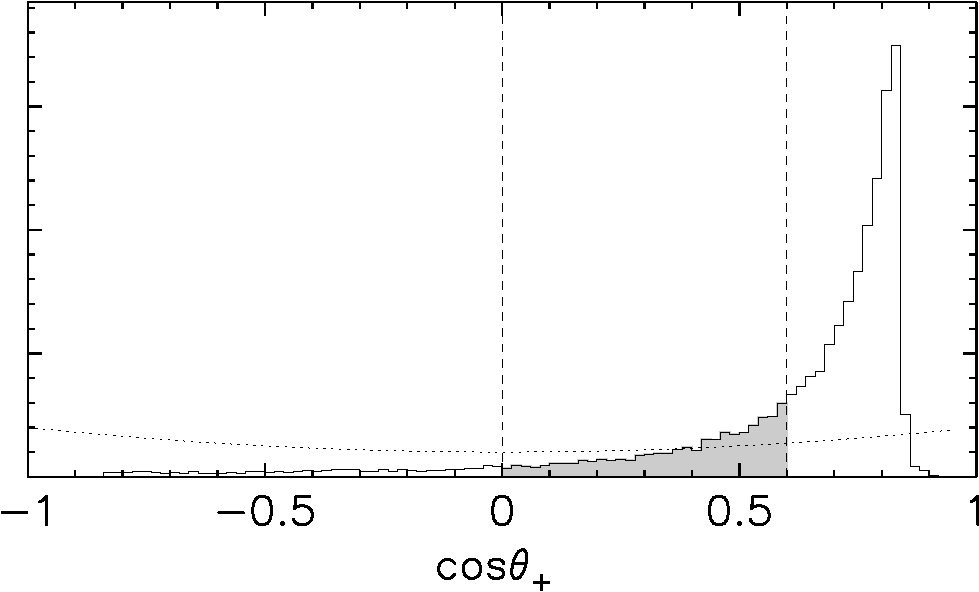
\includegraphics[width=10 cm]{/home/mccann/antithesis/plots/draw_innerbb} &
    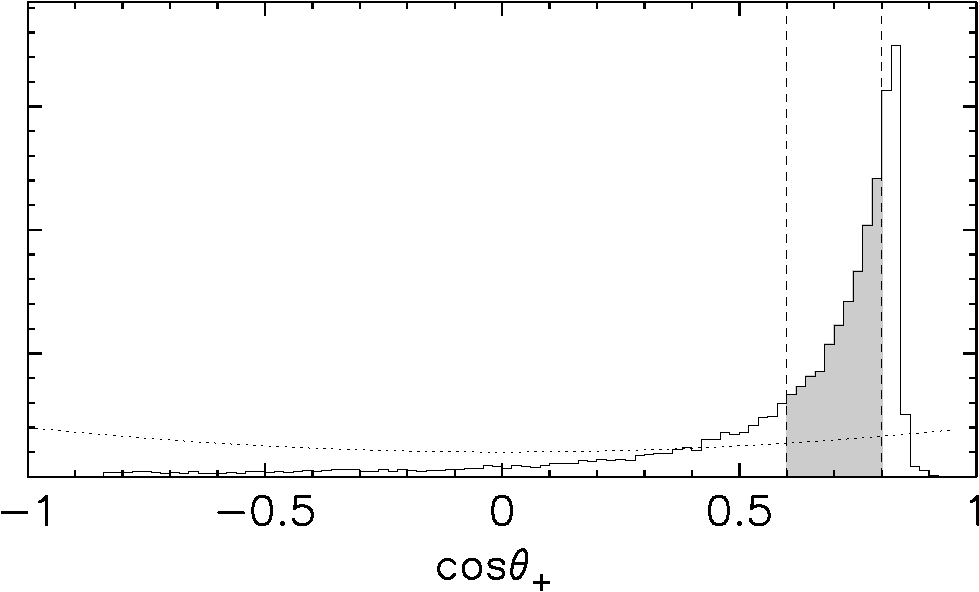
\includegraphics[width=10 cm]{/home/mccann/antithesis/plots/draw_outerbb} \\
    More contaminated by $\Upsilon \to e^+e^-$ &
    Less contaminated by $\Upsilon \to e^+e^-$
  \end{tabular}
\end{center}

\end{slide}

\begin{slide}[$e^+e^-$ Correction]

\[ \mbox{\#$e^+e^-$ to subtract} = \sigma_\Upsilon(E) \mbox{ } \mathcal{B}_{\mu\mu} \mbox{ } \frac{\displaystyle \int_{0.6}^{0.8} \cos^2\theta \, d\cos\theta}{\displaystyle \int_{-1}^{1} \cos^2\theta \, d\cos\theta} \mbox{ } \mathcal{L}_{\gamma\gamma} \]

\vfill $\sigma_\Upsilon(E)$ is the output of Karl's function (with
appropriate normalization), which includes interference between a
constant continuum process ($\mathcal{A}_{BB} = \sqrt{\sigma_{BB}}$)
and the Breit-Wigner ($+$ beam energy spread convolution)

\vfill
\begin{center}
  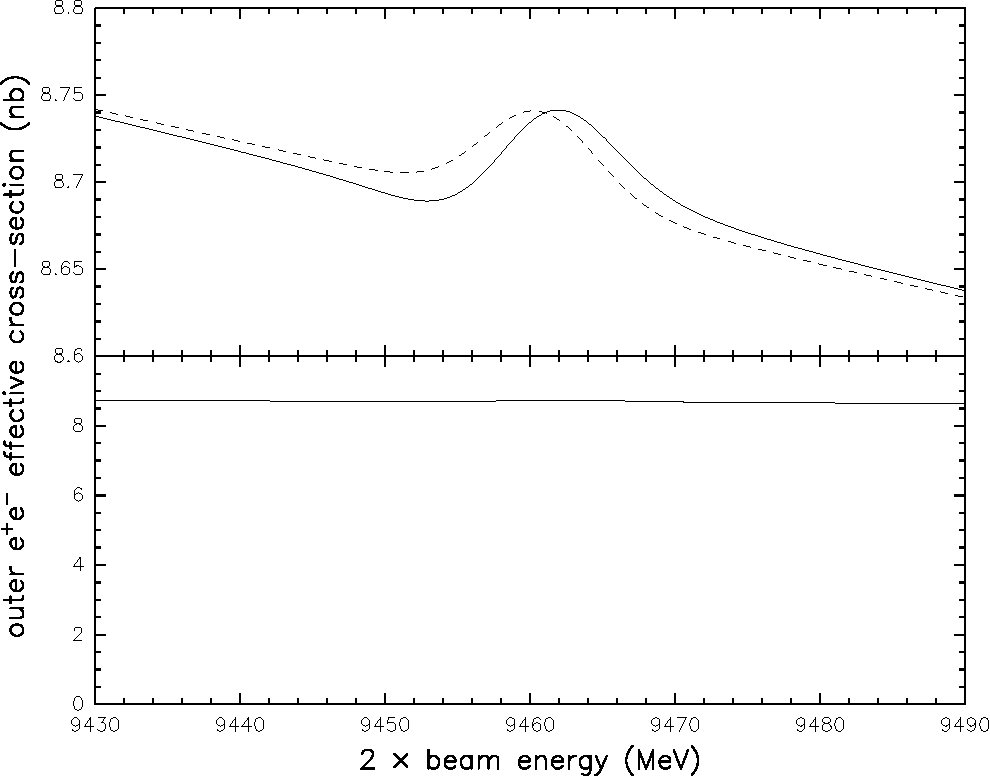
\includegraphics[width=0.5\linewidth]{/home/mccann/antithesis/plots/bbout_effective_crosssection}
\end{center}

\end{slide}

\begin{slide}[Systematic Uncertainties ($\Upsilon(1S)$)]

\begin{center}
  \renewcommand{\arraystretch}{2}
  \begin{tabular}{r c c}
               & area (MeV nb) & $\chi^2/ndf$ \\\hline
    Gamgam fit & 317.8 $\pm$ 2.2 & 214.1/(210-18) = 1.12 \\
    Inner Bhabha fit & 324.00 $\pm$ 1.2 & 259.9/(210-18) = 1.35 \\
    Outer Bhabha fit & 323.16 $\pm$ 0.95 & 257.2/(210-18) = 1.34 \\
    Restricted$^*$ Gamgam fit & 321.4 $\pm$ 1.1 & 240.3/(210-2) = 1.16 \\
  \end{tabular}
\end{center}

\vfill
$^*$Restricted fit doesn't allow week-by-week beam energy and beam
energy spread corrections to float: they are fixed to the outer Bhabha values.

\vfill Full Gamgam fit has week-by-week parameter outputs which are
consistent (some of them 2$\sigma$, I haven't done this
carefully\ldots) with Outer Bhabha fit--- a subtlety not caught by MINOS?

\vfill
\begin{center}
(THIS SLIDE IS TOO LATE-BREAKING TO BE CONSIDERED FINAL)

I'M STILL THINKING ABOUT THIS.
\end{center}

\end{slide}

\begin{slide}[What can we see with this high precision?]

With all scan data near the $\Upsilon(1S)$ peak:

\vfill
\begin{center}
  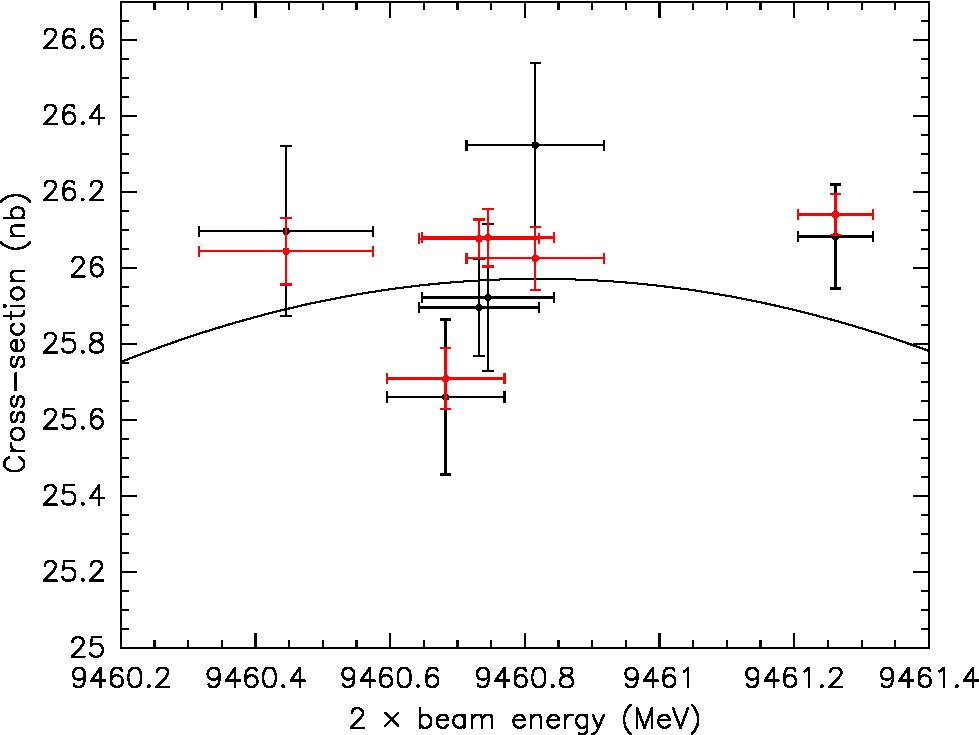
\includegraphics[width=0.8\linewidth]{/home/mccann/antithesis/plots/stability4_48hour}
\end{center}

\vfill
a 1.5\% excess in April $\Upsilon(1S)$.

\end{slide}

\begin{slide}[What can we see with this high precision?]

With all CLEO-III data near the $\Upsilon(1S)$ peak:

\vfill
\begin{center}
  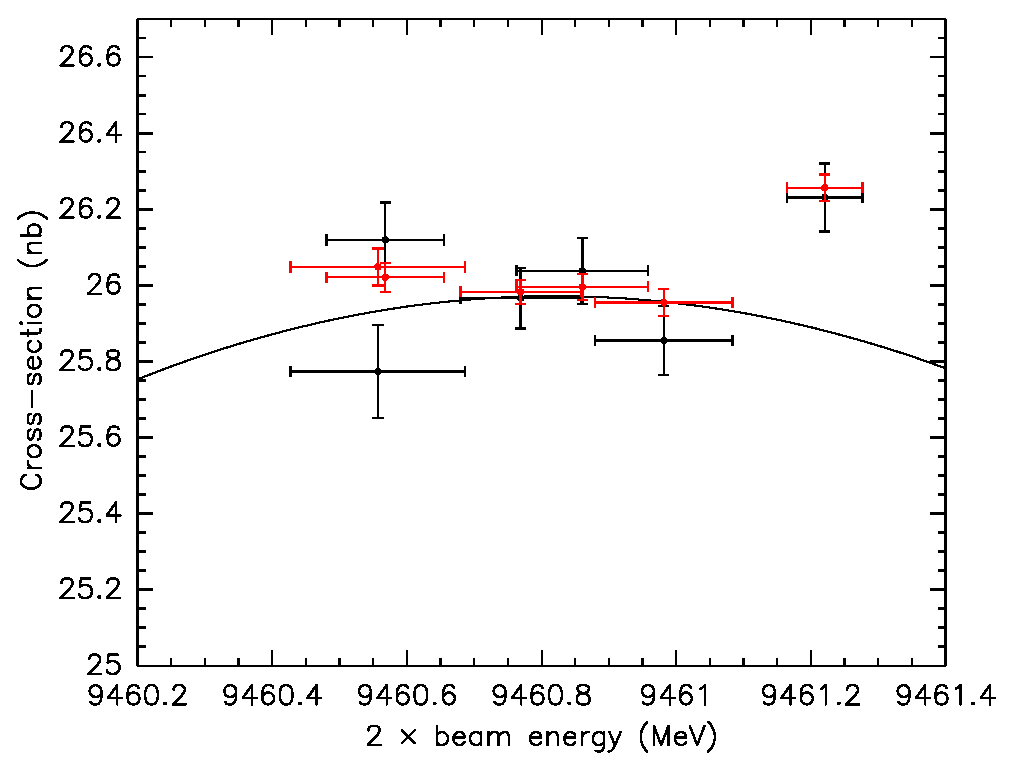
\includegraphics[width=0.8\linewidth]{/home/mccann/antithesis/plots/stability4_unlimited}
\end{center}

\vfill
a clear 1.5\% excess in April $\Upsilon(1S)$.

\end{slide}

\begin{slide}[What does this excess look like?]

In all distributions (visible energy is questionable), the excess is
distributed like $\Upsilon$ events.

\vfill
\begin{center}
  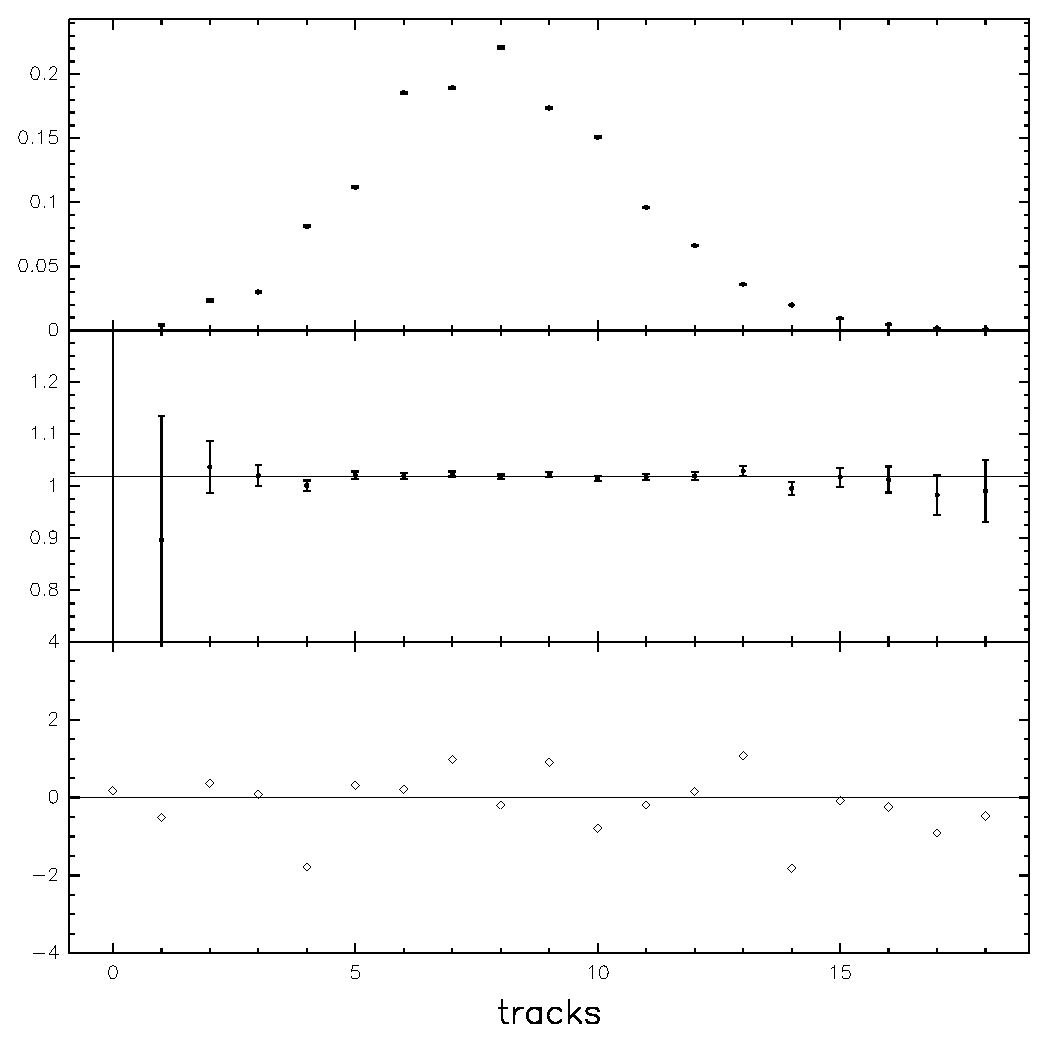
\includegraphics[width=0.6\linewidth]{/cdat/daf9/mccann/synthesis/rootstab_home/rootstab9_tracks}
\end{center}

$\rightarrow$ not an inefficiency or background, a narrowing of $\Upsilon$ beam energy spread?

\end{slide}

\begin{slide}[CESRV simulations]

Plausibly.

\vfill CESRV simulation of April vs.\ other weeks' savesets (0.93
correlation with measured beam energy spread)

\begin{center}
  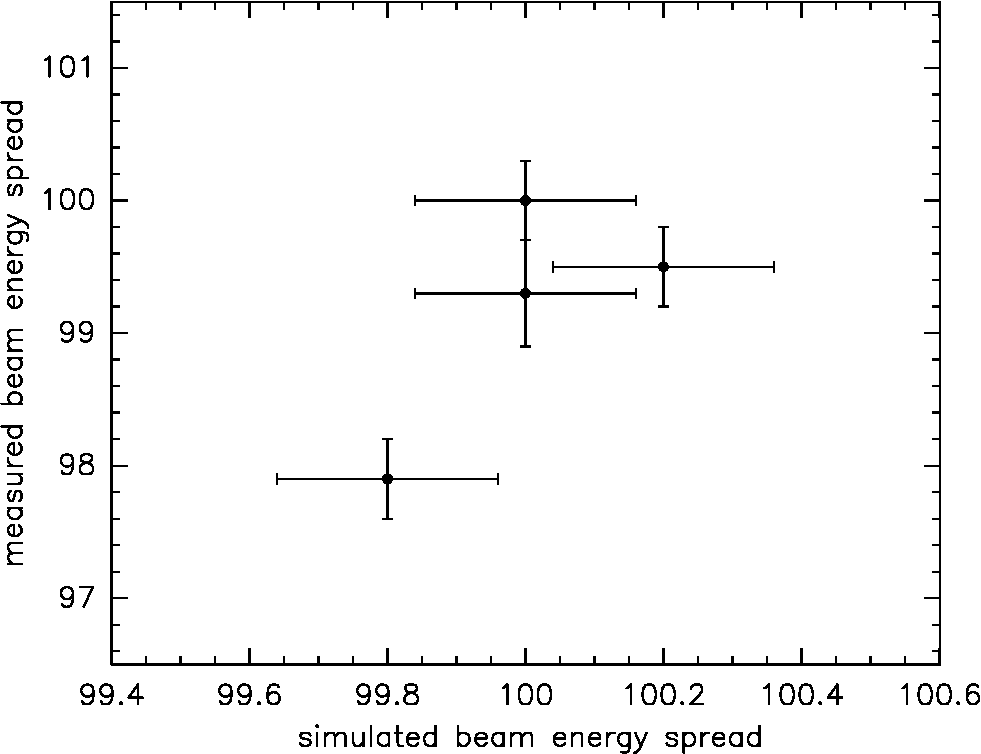
\includegraphics[width=0.5\linewidth]{/home/mccann/antithesis/plots/cesrv_correlation}
\end{center}

\vfill CESRV simulation of April vs.\ other weeks' orbits (physical
conditions) $\to$ 1\% discrepancy

\vfill So I will allow different beam energy spreads to float in
different weeks (surveyed CESR e-log to find the best breakpoints)

\end{slide}

\end{document}
